\begin{figure}[!ht]
\centering
\resizebox{1.0\columnwidth}{!}{
\begin{tabular}{c@{\hskip 7ex}c}
 %%%%%%%%%%%%%%%%%%%%%%%%%%%%%%A projection graph with two connected components %%%%%%%%%%%%%%%%%%%%%%%%%%%%%%
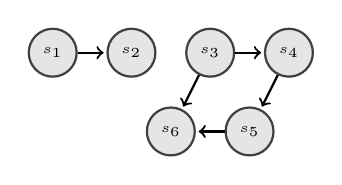
\begin{tikzpicture}[shorten >=1pt,->,scale=0.5]  
        \tikzstyle{sentence}=[circle,thick,draw=black!75,fill=black!10,minimum size=5mm]
        \tikzstyle{edge}=[draw, thick]
       \begin{scope}
         \node [sentence] (s1) at (0,2) {\tiny{$s_1$}};
         \node [sentence] (s2) at (2,2) {\tiny{$s_2$}};
         \node [sentence] (s3) at (4,2) {\tiny{$s_3$}}; 
         \node [sentence] (s4) at (6,2) {\tiny{$s_4$}}; 
         \node [sentence] (s5) at (5,0) {\tiny{$s_5$}}; 
         \node [sentence] (s6) at (3,0) {\tiny{$s_6$}}; 
         
         \path[edge] (s1) edge [above] node[font=\tiny] {} (s2);
         \path[edge] (s3) edge [above] node[font=\tiny] {} (s4);
         \path[edge] (s3) edge [above] node[font=\tiny] {} (s6);
         \path[edge] (s4) edge [above] node[font=\tiny] {} (s5);
         \path[edge] (s5) edge [above] node[font=\tiny] {} (s6);
         
        \end{scope}        
      \end{tikzpicture}
&
%%%%%%%%%%%%%%%%%%%%%%%%%%%%%% A projection with one component %%%%%%%%%%%%%%%%%%%%%%%%%%%%%%
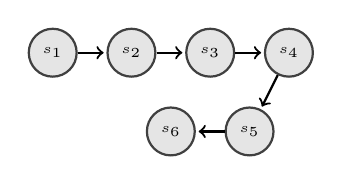
\begin{tikzpicture}[shorten >=1pt,->,scale=0.5]  
        \tikzstyle{sentence}=[circle,thick,draw=black!75,fill=black!10,minimum size=5mm]
        \tikzstyle{edge}=[draw, thick]
       \begin{scope}
         \node [sentence] (s1) at (0,2) {\tiny{$s_1$}};
         \node [sentence] (s2) at (2,2) {\tiny{$s_2$}};
         \node [sentence] (s3) at (4,2) {\tiny{$s_3$}}; 
         \node [sentence] (s4) at (6,2) {\tiny{$s_4$}}; 
         \node [sentence] (s5) at (5,0) {\tiny{$s_5$}}; 
         \node [sentence] (s6) at (3,0) {\tiny{$s_6$}}; 
         
         \path[edge] (s1) edge [above] node[font=\tiny] {} (s2);
         \path[edge] (s3) edge [above] node[font=\tiny] {} (s4);
         \path[edge] (s2) edge [above] node[font=\tiny] {} (s3);
         \path[edge] (s4) edge [above] node[font=\tiny] {} (s5);
         \path[edge] (s5) edge [above] node[font=\tiny] {} (s6);
         
        \end{scope}        
      \end{tikzpicture}
\\
\scriptsize{(a)} & \scriptsize{(b)}

\end{tabular}
}
\caption{Two graphs with the same outdegree value. Graph (a) has two
  components. It is less coherent. }
\label{f:con_com_projection}

\end{figure}